\section{Описание практической части}
\label{sec:Chapter4} \index{Chapter4}

После того, как все большие задачи из \autoref{sec:Chapter1} были разбиты на подзадачи, которые можно рассматривать непосредственно, перейдем к описанию их решения.

Чтобы удовлетворить требованию предоставить возможность обертки библиотеки в языки более высокого уровня, для написания публичного интерфейса был выбран язык \texttt{C}. Главным плюсом этого языка в данном случае является наличие нативных интерфейсов для него у многих современных языков программирования. Примером таких интерфейсов может служить \texttt{JNI} (\texttt{Java~Native~Interface}) \cite{jni} у языка \texttt{Java} или \texttt{N-API} (\texttt{Node~API}) \cite{napi} для языка \texttt{JavaScript}. Данные интерфейсы позволяют пользователю писать код, изменяющий параметры время исполнения. Например, \texttt{JNI} позволяет регистрировать функции, написанные на языке \texttt{C}, в качестве встроенных (\texttt{native}) функций платформы, которые в последствии можно вызывать из языка \texttt{Java}.

Поскольку для написания пользовательского интерфейса был выбран язык \texttt{C}, в котором нет возможности явно указывать приватные и публичные поля структур, то было принято решение имплементировать все сущности библиотеки как непрозрачные указатели. Эта техника позволяет разработчикам библиотеки не открывать пользователям деталей имплементации структур, вынуждая их использовать исключительно предоставленный библиотекой интерфейс. Необходимый эффект достигается путем вынесения определений структур в исходные файлы, что оставляет только декларации в заголовочных файлах. Таким образом, пользователь, подключивший себе заголовочный файл библиотеки, имеет только декларации библиотечных типов, в то время как имплементация библиотеки имеет доступ к полноценным определениям. Однако у данной техники есть один большой недостаток - отсутствие value-семантики у библиотечных типов в пользовательском интерфейсе. Действительно, поскольку пользователю недоступны определения типов, то пользовательский интерфейс может содержать только указатели на них. В рамках языка \texttt{C} это приводит к дополнительным вопросам про владение указаелем: кто аллоцировал память для объекта по указателю и чья обязанность ее освободить? В рамках данной библиотеки было решено проводить все аллокации строго на внутренних аренах библиотеки, и выдавать пользователю указатели на них. Это снимает с пользователя необходимость что-либо аллоцировать или освобождать на своей стороне для работы с интерфейсом библиотеки.

Общая архитектура библиотеки представлена на \autoref{fig:libScheme}.

\begin{figure}[h]
\centering
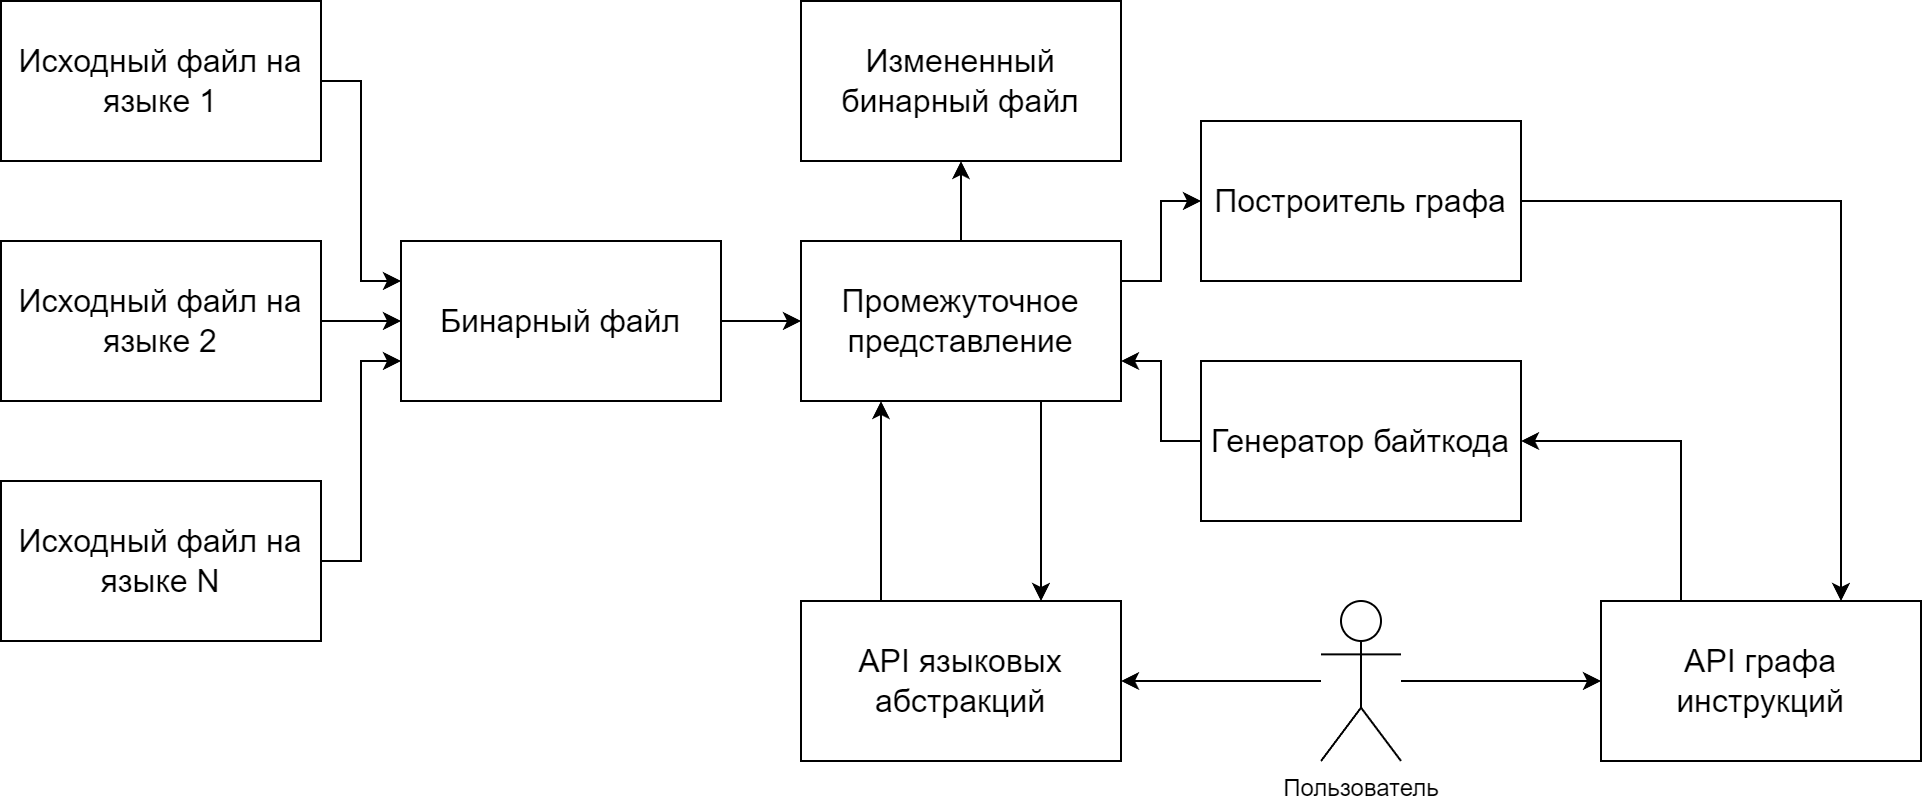
\includegraphics[width=.8\textwidth]{library_scheme.png}
\caption{Общая схема работы библиотеки.}
\label{fig:libScheme}
\end{figure}

Входной точкой пользовательского интерфейса библиотеки является бинарный файл. Он может быть получен после компиляции пользователем кода при помощи любого из возможных фронтендов платформы. Во время загрузки библиотекой бинарного файла происходит построение промежуточного представления всех структур, овеществялющих языковые абстракции, закодированные в бинарном файле. Далее, пользователь имеет возможность работать с этим представлением посредством двух интерфейсов. Первый позволяет работать с метаданными файла, такими как типы, определения функций и другие. Второй интерфейс служит для работы с телами функций, а также бинарными инструкциями.

\subsection{Фронтенд}

Для начала кратко опишем архитектуру фронтенда многоязыковой платформы, в рамках которой разрабатывается описываемая библиотека. Рассмотрим то, каким образом генерируется бинарный файл, какова его структура, и как он в дальнейшем исполняется.

Для того чтобы поддержать исполнение нескольких языков программирования в рамках одной плафтормы, необходимо решить задачу компиляции их исходных и бинарных файлов в представление, поддерживаемое платформой. С этой целью на платформе были имплементированы несколько фронтендов, каждый из которых компилирует исходный или бинарный входной файл в бинарный формат платформы. Благодаря единому бинарному формату в рамках платформы становится возможным написание таких инструментов, как описанный в данной работе, а также достигается бесшовная интероперация между различными языками.

Однако для эффективных компиляции и исполнения различных языков требуется разный по семантике набор бинарных инструкций. Это требование возникает из-за отличного поведения сущностей во время компиляции и во время исполнения. Проиллюстрируем это рассмотрением двух больших групп исполняемых на виртуальных машинах (\texttt{managed}) языков: статических и динамических. Примером статического \texttt{managed} языка могут являться \texttt{Java} или \texttt{Kotlin}. Данные языки статически типизированы, тоесть тип в них не является частью значения, поэтому например все обращения к полям объектов в них могут быть вычислены во время компиляции кода. Это позволяет компилятору и загрузчику осущесвтлять множество анализов и верифицировать код на предмет выполнения языковых гарантий, таких как связанные с модификаторами доступа сущностей. Для поддержки возможности верификации кода даже после компиляции исходных файлов требуется сохранение всей необходимой информации на уровне бинарных инструкций, что влияет на проектирование набора инструкций в виртуальных машинах, исполняющих эти языки программирования. Рассмотрим процесс обращения к полю класса в языке \texttt{Java}. Скомпилировав код, показанный в \autoref{lst:javaSource} компилятором \texttt{JVM} получим последовательность бинарных инструкций, показанную в \autoref{lst:javaBc}.

\begin{lstlisting}[language=Java, caption=Исходный код языка \texttt{Java}., label=lst:javaSource]
    public class MyClass {
        public int a = 1;
        public static int b = 2;
    };
    public class Main {
        public static void main() {
                MyClass my = new MyClass();
                int res = my.a + MyClass.b;
        }
    }
\end{lstlisting}

\begin{lstlisting}[caption=Бинарный код виртуальной машины \texttt{JVM}., label=lst:javaBc]
    public class MyClass
    public int a;
        descriptor: I
        flags: ACC_PUBLIC
    public static int b;
        descriptor: I
        flags: ACC_PUBLIC, ACC_STATIC

    public class Main
    Constant pool:
        ...
        #7 = Class #8 // MyClass
        #8 = Utf8 MyClass
        ...
        #10 = Fieldref #7.#11 // MyClass.a:I
        #11 = NameAndType #12:#13 // a:I
        #12 = Utf8 a
        #13 = Utf8 I
        #14 = Fieldref #7.#15 // MyClass.b:I
        #15 = NameAndType #16:#13 // b:I
        #16 = Utf8 b
        ...
    public static void main();
        ...
        getfield #10 // Field MyClass.a:I
        getstatic #14 // Field MyClass.b:I
        iadd
        ...
\end{lstlisting}

Как видно из листинга бинарного кода \autoref{lst:javaBc}, обращения к полям класса \texttt{MyClass} в методе \texttt{main} имеют всю необходимую типовую информацию, необходимую для проверок даже после компиляции. Действительно, поскольку аргументом инструкций доступа к полю является полный дескриптор необходимого поля, загрузчик имеет возможность найти это поле среди загружаемых классов и проверить все флаги доступа. Подобное проектирование инструкций позволяет имплементировать безопасное и надежное исполнение программ даже после применения к коду бинарных манипуляций.

Классическим примером динамического managed языка программирования является \texttt{JavaScript}. Поскольку этот язык динамический, тип в нем является частью значения переменной, и не может быть выведен фронтендом во время компиляции. Более того, из-за того, что объект в данном языке - это коллекция пар ключ-значение, из который можно как удалять, так и добавлять пары, то ни о какой верификации инструкций во время загрузки не может быть и речи. Более того, меняется семантика доступа к полю объекта, что находит свое отражение в наборе инструкций, которым оперируют виртуальные машины, исполняющие данный язык. Проиллюстрируем отличия в семантике достпа к полю объекта на примере бинарного кода виртуальной машины машины \texttt{V8}. Написав код, аналогичный \autoref{lst:javaSource}, получим следующий результат.

\begin{lstlisting}[language=Javascript, caption=Исходный код языка \texttt{JavaScript}., label=lst:jsSource]
    class MyClass {
        static a = 1;
        b = 2;
    }
    function main() {
        let my = new MyClass();
        let res = my.b + MyClass.a
    }
    main()
\end{lstlisting}

\begin{lstlisting}[caption=Бинарный код виртуальной машины \texttt{V8}., label=lst:jsBc]
    [generated bytecode for function: main (0x0e93e5d98a29 <SharedFunctionInfo main>)]
    Constant pool
        ...
        0: ... <String[7]: #MyClass>
        1: ... <String[1]: #b>
        2: ... <String[1]: #a>
        ...
    Bytecode
        ...
        ThrowReferenceErrorIfHole [0]       // #MyClass
        Star2
        Construct r2, r0-r0, [0]
        Star0
        GetNamedProperty r0, [1], [3]       // #b
        Star2
        LdaImmutableCurrentContextSlot [2]
        ThrowReferenceErrorIfHole [0]       // #MyClass
        Star3
        GetNamedProperty r3, [2], [5]       // #a
        Add r2, [2]
        ...
\end{lstlisting}

Как видно из \autoref{lst:jsBc}, в динамическом языке совершенно другая семантика обращения к полю. Во-первых, обращение к статическому и к динамическому полю выражается единой инструкцией - \texttt{GetNamedProperty}. Во-вторых, никакой информации, которая могла бы быть полезна при верификации не может быть сохранено и не сохраняется в виду модели объекта в данном языке. Также, поскольку в динамических языках тип является свойством значения, в общем случае фронтенд не может вывести, что складываются два целочисленных значения. Поэтому в отличие от \texttt{Java}, где использовалась специализированная инструкция \texttt{addi}, в \autoref{lst:jsBc} используется общая операция \texttt{Add}.

В виду этих и еще многих различий семантик исполнения различных языков, на платформе имплементировано несколько расширяемых наборов инструкций (\texttt{ISA}), каждый из которых исполняется на одной из виртуальных машин платформы в зависимости от исходного языка приложения.

Поскольку приложения могут быть написаны на нескольких языках программирования, то после линковки всех бинарных файлов приложения может оказаться так, что в рамках одного бинарного файла будет присутствовать бинарное представление сущностей из разных языков.

Это является большой проблемой для пользователей, пытающихся прочитать и проинтерпретировать бинарный файл, поскольку разные фронтенды могут по-разному кодировать необходимые ему языковые сущности в рамках одного бинарного формата. Так например фронтенду для виртуальной машины, имплементирующей спецификацию языка \texttt{JavaScript} \texttt{ECMA-262} нет смысла кодировать пользовательский класс никак иначе, кроме как функцию, в то время как фронтенду языка \texttt{Java} нет смысла кодирвать класс иначе как структуру с фиксированными разметкой и модификаторами доступа. Аналогично, фронтенду языка \texttt{JavaScript} нет необходимости сохранять информацию о типах или о сигнатурах функций, но для исполнения языка \texttt{Java} эта информация является критичной. Кроме того, некоторые фронетнды могут использовать структуры бинарных файлов для хранения имплементационных деталей, не имеющих прямого отображения на исходный код. Таким образом мы получаем ситуацию, когда каждая сущность в бинарном файле может быть интерпретирована по-разному в зависимости исходного языка и использованного фронтенда. Отсюда возникает требование скрыть такие сложные детали имплементации бинарного формата от пользователя.

Далее будут отдельно рассмотрены две части пользовательского интерфейса: интерфейс для работы с метаданными бинарного файла и интерфейс для работы с бинарными инструкциями. При рассмотрении каждого из них будет представлена его архитектура, а также то, как ее имплементация решает обговоренные выше подзадачи. Подробно в данной работе будет рассмотрен только интерфейс для работы с метаданными файла.

\subsection{Интерфейс для работы с метаданными бинарного файла}

Как уже было сказано ранее, для имплементации интерфейса для работы с метаданными бинарного файла был выбран уровень абстракции языковых сущностей. Данное решение было продиктовано желанием скрыть от пользователей платформы сложное устройство бинарного файла, а также убрать необходимость пользователю разбираться в деталях имплементации различных фронтендов платформы.

Однако данное решение требует аккуратного выбора набора языковых сущностей, с которыми будет работать библиотека, поскольку их должно быть достаточно чтобы выразить все необходимые языковые абстракции поддерживаемых языков, но при этом они должны быть достаточно общими, чтобы не создавать ситуации, когда пользователь путается, какую языковую сущность ему необходимо применить в том или ином случае.

Для выделения таких сущностей было проведено сравнение распространенных managed языков программирования. Сравнение проводилось в два этапа: сначала языки сравнивались по набору поддерживаемых языковых сущностей, затем сравнивалась их семантика: какие операции к ним применимы, а какие - нет.

В результате сравнения языков \texttt{JavaScript}, \texttt{TypeScript}, \texttt{Java}, \texttt{Kotlin} и нативного статического языка платформы был выделен следующий набор сущностей, достаточный для того, чтобы оперировать этими языками.

\begin{itemize}
    \item Класс (\texttt{Class}) - общее обозначение для всех структур данных.
    \item Функция (\texttt{Function}) - общее обозначение для всех видов функций. Анонимных функций, методов, свободных функций и дргуих.
    \item Поле (\texttt{Field}) - общее обозначение для полей чего-либо. Класса, интерфейса, пространства имен и других.
    \item Перечисление (\texttt{Enum}) - обозначение для типов перечисления.
    \item Пространство имен (\texttt{Namespace}) - обознчание для пространств имен.
    \item Аннотация (\texttt{Annotation}) и Декоратор (\texttt{Decorator}) - являются взаимоисключающими понятиями, поскольку обозначают статический и динамический механизмы добавления метаданных к декларациям.
\end{itemize}

Поскольку, как уже было обозначено ранее, один бинарный файл может содержать сущности из нескольких разных языков, в рамках библиотеки было решено адаптировать следующую модель бинарного файла. Бинарный файл - это коллекция сущностей, называемых модуль (\texttt{Module}). Модуль же - это именованная коллекция языко-специфичных деклараций, у которой есть свой публичный интерфейс, и свой список внешних зависимостей. Поскольку каждый язык имеет собственный механизм работы с внешними зависимостями, а также способ обозначения публичного интерфейса, было решено ввести абстракиции, обобщающие понятия внешней зависимости и сущности из публичного интерфейса модуля. Ими являются дескриптор импорта \texttt{Import~Descriptor} и дескриптор экспорта \texttt{Export~Descriptor}. Целью введения этих дескрипторов является отделение понятия внешней зависимости и публичного интерфейса от языко-специфичной нагрузки и предоставление некоего общего интерфейса для работы с ними, оставив при этом возможность работать с ними в контексте конкретного языка. С помощью понятий модуль, дескриптор импорта и дескриптор экспорта возможно описать общий механизм отношений между модулями и сущнстями из модулей, что позволяет библиотеке единообразно обрабатывать сценарии интероперабельности и сценарии работы с внешними зависимостями в рамках одного языка. Данный механизм является строго необходимым, поскольку различия в механизмах взаимодействия с внешними сущностями у различных языков во время компиляции и во время исполнения могут радикально отличаться. Так, например, для языка \texttt{Java} каждая импортируемая сущность может быть разрешена в класс, метод или поле класса во время компиляции проекта. После чего данные сущности могут быть сохранены в бинарном файле с пометкой \texttt{external}. Во время исполнения программы будут загружены класс-файлы с их определениями и код будет иметь возможность быть исполеннным. Из-за такой имплементации работы с внешними сущностями, на инструкций работа с внешним и локальным классом абсолютно не отличается. Однако для такого языка как \texttt{JavaScript} ни о каком разрешении имен до начала времени исполнения речи идти не может, поэтому вся информация о внешних зависимостях и публичном интерфейсе согласно спецификации \texttt{ECMA-262} хранится в отдельной для каждого модуля таблице. Данный подход очевидно отражается на наборе инструкций, с которыми работает виртуальная машина, имплементирующая данную спецификацию. Среди них появляются инструкции, работающие непосредственно с вхождениями в этой таблице. Целью введения понятий дескриптора импорта и дескриптора экспорта как раз и является сокрытие подобных деталей имплементации от пользователя и вынесение понятий внешней зависимости и публичного интерфейса модуля в языко-независимую чать библиотеки, чтобы упростить интерфейс работы с интероперабельностью.

Также, чтобы отразить факт того, что поддерживаемые платформой языки будут скомпилированы в один из ограниченного числа наборов инструкций, поддерживаемых виртуальными машинами платформы, было введено понятие \texttt{Target}, соединяющее в себе как исходный язык, так и спользуемый при его компиляции набор инструкций. Например один и тот же код на языке \texttt{Java} может быть представлен совершенно разными наборами инструкций на разных платформах, таких как \texttt{JVM} и \texttt{ART}. В рамках нашей библиотеки этот факт отразился бы в определении двух \texttt{Target}-ов для языка \texttt{Java}: \texttt{lib\_Core\_Target\_Java\_ART} и \texttt{lib\_Core\_Target\_Java\_JVM}.

Анализ семантики выделенных выше языковых сущностей показал, что функционал, применимый к данным сущностям можно разбить на две основные группы: общий и языко-специфичный.

Общий функционал над сущностями библиотеки имеет одно и то же семантическое значение для всех языков. Например взятие имени у функции или у класса. Также, в общий функционал входят те функции, для которых можно однозначно определить поведение во всех языках. В них входят функции-перечислители, принимающие функцию-посетитель в качестве аргумента (как например функция \texttt{ClassEnumerateFields} или \texttt{ClassEnumerateMethods}). Для языков, в которых данные операции имеют смысл (например \texttt{Java}), происходит вызов функции-посетителя, а для языков, в которых операции смысла не имеют (например \texttt{JavaScript}), просто ничего не происходит, и функция-посетитель не вызызвается ни разу.

Таким образом, основная часть пользовательского интерфейса состоит из следующих сущностей:

\begin{itemize}
    \item Объявления всех библиотечных типов. В эти объявления входят как служебные типы, такие как тип, строка и тп, так и обозначенные выше языковые сущности. Всем подобным типам соответствуют имена вида \texttt{lib\_Core\_XXX}, где \texttt{Core} означает принадлежность к основной части интерфейса, а \texttt{XXX} заменяется на имя сущности, описываемой типом, например \texttt{lib\_Core\_Class} или \texttt{lib\_Core\_Type}.
    \item Все функции-перечислители для объявленных типов. Поскольку поведение таких функций было однозначно определено выше для всех возможных языков, они могут стать частью общего интерфейса.
    \item Все функции-геттеры, для которых возможно определить однозначеное поведение для всех возможных языков.
    \item Интерфейс для модификации всех языко-независимых сущностей: \texttt{lib\_Core\_File}, \texttt{lib\_Core\_String}, \texttt{lib\_Core\_Type}, \texttt{lib\_Core\_Value} и других.
\end{itemize}

Задачей языко-специфичного интерфейса является определить, какие из основных сущностей релевантны для конкретного языка, а также определить функционал, применимый только к ним. Языко-специфичный интерфейс состоит из множества языковых расширений, каждое из которых определяет специфику отдельного языка. Каждое расширение определяет свой набор \texttt{lib\_<LANG>\_XXX} сущностей, специализирующих \texttt{lib\_Core\_XXX} сущности из основной части библиотеки. Каждое из расширений определяет только те сущности, которые ему нужны. Так, например, расширению \texttt{JavaScript} не нужно будет определять свой \texttt{lib\_JavaScript\_Field}, поскольку понятие поля в данном расширении не имеет смысла. Таким образом, внутренняя имплементация структуры \texttt{lib\_Core\_Class} будет выглядеть следующим образом:

\begin{lstlisting}[language=Java, caption=Внутренняя имплементация типа \texttt{lib\_Core\_Class}, label=lst:libClass]
    struct lib_Core_Class {
        /* Used to determiine correct type of `impl`. */
        lib_Core_Module* m;
        /* ... */
        union {
            lib_JS_Class* JS;
            lib_Java_Class* Java;
            /* ... */
        } impl;
    };
\end{lstlisting}

Расширения, как уже было сказано выше, определяют языко-специфичный функционал только над специализированными сущностями из основной части интерфейса. Каждое расширение имплементирует языковой инстерфейс для одного или более \texttt{Target}-ов, поскольку языковые метаданные определяются исходным языком, а не выбранным набором инструкций. Для работы с функционалом расширения пользователям необходимы функции-конверторы между сущностями основной части и сущностями расширения:

\begin{lstlisting}[language=Java, caption=Пример функций-конверторов., label=lst:libConvertors]
    struct lib_Java_Api {
        /* ... */
        CoreClassGetJavaClass,  // Converts lib_Core_Class* to lib_Java_Class*
        JavaClassGetCoreClass,  // Converts lib_Java_Class* to lib_Core_Class*
        /* ... */
    };
\end{lstlisting}

Поскольку большая часть модификаций сущностей требует языко-специфичного набора параметров, в рамках библиотеки было решено вынести весь интерфейс для модификации языковых сущностей в расширения, где модификации будут определены для канкретных специализаций \texttt{lib\_<LANG>\_XXX}.

Также, языковые расширения содержат методы для инспекции метаданных всех \texttt{lib\_<LANG>\_XXX} сущностей, поскольку большая часть метаданных является языко-специфичной, и для функций-геттеров невозможно определить общего поведения. Функции-геттеры, вынесенные в основную часть не дублируются в расширении.

Поскольку механизм работы с внешними сущностями определяется парой языков (экспортируемый-экспортирующий или импортируемый-импортирующий), каждое расширение должно предоставить собственный интерфейс для работы с импортами и экспортами. Этот интерфейс должен включать в себя добавление и удаление внешних зависимостей, а также добавление и удаление сущностей из публичного интерфейса модуля. Еще одной важной частью интерфейса является извлечение из дескрипторов языко-специфичных данных. Так, для языка Java мы можем извлечь из дескриптора импорта \texttt{lib\_Java\_Class}, \texttt{lib\_Java\_Field}, \texttt{lib\_Java\_Function}. Тем самым, каждое расширение определяет возможности своего языка к интероперабельнсти, задавая пары языков, между которыми возможно построение отношений экспорт-импорт или импорт-экспорт. Это позволяет определять правила преобразований между различными механизмами работы с внешними сущностями в частном порядке для каждой конкретной пары.

Резюмируя сказанное выше, роль языковых расширений состоит в следующем: основная часть пользовательского интерфейса для работы с метаданными предоставляет общий интерфейс, позволяющий писать общий код для работы с любым исходным языком; этот интерфейс строится поверх внутренних и публичных функций расширений. Расширения предоставляют языко-специфичный функционал, работающий только с сущностями из расширения.

Ниже представлен пример того, как может выглядеть расширение для языка \texttt{TypeScript}.

\begin{lstlisting}[language=Java, caption=Примерный код расширения \texttt{Typescript}., label=lst:libTsExtension]
    /* Declaring language-specific entities. */
    struct lib_TS_Module;
    struct lib_TS_Class;
    struct lib_TS_Function;
    struct lib_TS_Decorator;
    struct lib_TS_Namespace;
    /* etc. */

    struct lib_Api_TS
    {
        /* lib_TS_Module */
        /*
         * Note, how pair AddImport/AddExport defines,
         * which languages are supported for interop with extension's language.
         */
        ModuleAddImportFromJS(lib_TS_Module* importing, lib_JS_Module* imported, ... payload);
        ModuleAddExportFromJS(lib_TS_Module* exporting, lib_JS_Module* exported, ... payload);
        ModuleAddImportFromTS(lib_TS_Module* importing, lib_TS_Module* imported, ... payload);
        ModuleAddExportFromTS(lib_TS_Module* exporting, lib_TS_Module* exported, ... payload);
        /* etc. */
        ModuleRemoveImport(lib_TS_Module* m, lib_Core_ImportDescriptor* id);
        ModuleRemoveExport(lib_TS_Module* m, lib_Core_ExportDescriptor* ed);
        TSModuleGetCoreModule(lib_TS_Module* m),
        CoreModuleGetTSModule(lib_Core_Module* m),

        /* lib_TS_Namespace */
        TSNamespaceGetConstructorFunction(lib_TS_Namespace* ns),
        TSNamespaceGetCoreNamespace(lib_TS_Namespace* ns),
        CoreNamespaceGetTSNamespace(lib_Core_Namespace* ns),

        /* lib_TS_Enum */
        /* lib_TS_Class */
        /* lib_TS_Function */
        /* etc. */
    };
\end{lstlisting}

Комбинируя использование функций из общего интерфейса и функций из языко-специфичных расширений, пользователь может писать безопасную общкю логику, расширяемую по необходимости языко-специфичными действиями. Ниже приведен пример такого кода. Пусть перед пользователем стоит задача обойти все функции в бинарном файле. Он знает, что в языке \texttt{TypeScript} пространство имен представлено немедленно-вызываемой функцией \texttt{IIFE~(Immediately~Invoked~Function~Expression)}, которую пользователь также хочет обработать как обычную функцию. Данную логику можно выразить следующим образом:

\begin{lstlisting}[language=C, label=lst:getTsNamespace]
    static bool NamespaceEnumerator(lib_Core_Namespace* ns, void* data) {
        /* ... */

        /*
         * I, as user, know that TS namespace can contain expressions,
         * and this logic is not present in the `Core` part. So language-specific
         * behaviour is needed in order to process namespace's constructor.
         */
        lib_Core_Module* m = api_core->NamespaceGetModule(ns)
        if (lib_Core_Target_TS == api_core->ModuleGetTartget(m)) {
            auto ts_namespace = api_ts->CoreNamespaceGetTSNamespace(ns);
            auto ts_ns_ctor = api_ts->NamespaceGetConstructor(ts_namespace);
            auto ns_ctor = api_ts->TSFunctionGetCoreFunction(ts_ns_ctor);
            (void)FunctionEnumerator(ns_ctor, data);
        }

        /* ... */
    }
\end{lstlisting}


\subsection{Интерфейс для работы с бинарными инструкциями}

Как уже было сказано ранее, в рамках рассматриваемой платформы имплементировано несколько наборов инструкций, поддерживаемых различными виртуальными машинами. Все языки программирования, поддерживаемые на платформе транслируются в один из этих наборов инструкций в зависимости от используемого фронтенда. Каждый из имеющихся на платформе наборов инструкций является регистровым, с одним выделенным регистром, называемым аккумулятором, использующимся как неявный регистр для сохранения возвращаемого значения. Данный дизайн инструкций позволяет уменьшить размер инструкций за счет того, что нет необходимости кодировать регистр для возвращаемого значения, что приводит к уменьшению размера кода вцелом. Операндами инструкций могут являться как регистры, так и конкретные (\texttt{immediate}) значения.

Поскольку одним из требований к имплементации рассматриваемой библиотеки является удобство имплементации сложных анализов тел функций, что сводится к предоставлению пользователям механизмов для анализа потока управления и потока данных, в рамках библиотеки не было предложено интерфейса для работы с непосредственным представлением инструкций как они хранятся в бинарном файле. Действиетльно, для того, чтобы провести анализ потока управления или данными по последовательности регистровых инструкций пользователю придется писать на своей стороне весьма сложные анализы. Более того, если пользователь захочет добавить свою собственную инструкцию в последовательность, то ему придется писать свой алгоритм аллокации регистров, чтобы избежать конфликтов с уже используемыми. Чтобы избежать данных затруднений, было предложено переиспользовать компилятор платформы для предоставления пользовательского интерфейса для работы с телами функций. Данный компилятор является очень гибким, и уже успешно переиспользуется в имплементации \texttt{JIT}, \texttt{AOT} компиляторов, а также в имплементации оптимизатора бинарного кода.

Компилятор преобразует последовательность инструкций бинарного файла в \texttt{SSA} граф из них, попутно добавляя необходимые компилятору служебные инструкции. \texttt{SSA} граф является одинм из лучших представлений для анализа тел функций, поскольку анализ потока управления и анализ потока данных получаются бесплатно "из коробки", и именно на данном представлении проводится большинство описанных в литературе анализов. Еще одним преимуществом переиспользования компилятора является простота поддержки компиляторных проходов (например таких как построение дерева доминаторов) в пользовательском интерфейсе. Поскольку все они уже имплементированы для внутреннних нужд компилятора, библиотеке остается только написать безопасную для пользователя обертку.

Для отделения языко-независимой структуры графа от конкретных наборов инструкций, публичный интерфейс для работы с бинарными инструкциями был разделен на две основные части: интерфейс набора инструкций и интерфейс графа инструкций.

\subsubsection{Интерфейс графа инструкций}

Данный интерфейс является оберткой над интерфейсом компилятора. Как уже было сказано выше, данный интерфейс работает с графом инструкцйи в \texttt{SSA} форме. Остановимся на этотм моменте более подробно. \texttt{SSA} (\texttt{Single Static Assignment}) - вид промежуточного представления кода функции. основной особенностью \texttt{SSA} формы является то, что присвоение в каждую переменную в ней происходит лишь один раз, что значитеотно упрощает анализ потока данных. Еще дним важным свойством, присущим всем разновидностям SSA, вклю-
чая приведенное выше определение, является ссылочная прозрачность: поскольку для каждой переменной в тексте программы существует только одно определение, значение переменной не зависит от ее положения в программе.

Граф инструкций в \texttt{SSA} форме состоит из базовых блоков, которые образуют граф потока управления. Базовый блок - это линейный участок инструкций, в который можно попасть только через самую первую инструкцию, и не имеющий инструкций условного перехода, кроме самой последней Наличие понятия базового блока заметно упрощает анализ поттока управления функции.

Как видно из определения, данный граф не имеет привязки к какому-либо конкретному набору инструкций, поэтому интерфейс графа инструкций весьма прост:

\begin{itemize}
    \item Объявляет сущности \texttt{lib\_Core\_Graph}, \texttt{lib\_Core\_BasicBlock}, \texttt{lib\_Core\_Instruction}.
    \item Предоставляет функции для работы ними. Интерфейс для \texttt{lib\_Core\_Instruction} не содержит языковой специфики, состоит только из функций для инспекции и манипуляции входами (\texttt{inputs}) и пользователями (\texttt{users}) инстукций. По тем же причинам не включает в себя интерфейс для создания экземпляров инструкций, поскольку данные функции являются зависимыми от используемого набора инструкций.
\end{itemize}

\subsubsection{Интерфейс набора инструкций}

Для определения возможных наборов инструкций был выделен отдельный интерфейс для работы с ними. Данный интерфейс определяет набор инструкций как список функций-конструкторов, а также функций-геттеров и -сеттеров для получившихся экземпляров \texttt{lib\_Core\_Instruction}. Подобное разделение позволяет предоставить более понятный пользовательский интерфейс, а также изолировать проверки на то, что добавляемая инструкция соответствует набору инструкций, использующихся в графе в едином месте в имплементации.

Каждый из наборов инстукций в виду их специфики может представлять лишь ограниченное число языков, в связи с чем за каждым из интерфейсов для набора инструкций закреплен определенный и фиксированный список \texttt{Target}-ов, для которых он применим. Так, например, набор инструкций виртуальной машины, имплементирующей спецификацию \texttt{ECMA-262}, очевидно может быть применен для кодирования тел функций языков \texttt{JavaScript} и \texttt{TypeScript}. Чтобы сделать данную логику прозрачной для пользователя, в библиотеку были внесены функции, позволяющие опрашивать граф, каким набором инструкций он закодирован.

\begin{lstlisting}[language=C, label=lst:libIsaApi]
    /* include/graph_core.h */

    enum lib_Core_ISA {
        lib_Core_ISA_ISA1,
        lib_Core_ISA_ISA2,
        /* ... */
    };

    struct lib_Core_GraphApi {
        /* ... */
        GraphGetTarget,  // returns lib_Core_Target
        GraphGetIsaType,     // returns lib_Core_ISA
        /* ... */
    };
\end{lstlisting}

Данный функционал позволяет пользователям писать общий код для работы с графом, используя \texttt{Target}-специфичный интерфейс только по необходимости.

Таким образом, заголовочные файлы интерфейса для работы с набором инструкций выглядят примерно так:

\begin{lstlisting}[language=C, label=lst:libIsaApi]
    /* include/isa/isa_1.h */

    enum lib_Core_ISA1_Opcode {
        lib_Core_ISA1_Opcode_XXX,
        lib_Core_ISA1_Opcode_YYY,
        /* ... */
    };

    struct lib_Core_ISA1_Api {
        IsaGetIsaType,  // returns lib_Core_ISA

        InstCreateXXX,
        InstCreateYYY,
        /* ... */

        InstGetClass,
        InstGetString,
        /* ... */

        instSetClass,
        InstSetString,
        /* ... */
    };

    /* include/isa/isa_2.h */

    enum lib_Core_ISA2_Opcode {
        lib_Core_ISA2_Opcode_AAA,
        lib_Core_ISA2_Opcode_BBB,
        /* ... */
    };

    struct lib_Core_ISA2_Api {
        IsaGetIsaType,  // returns lib_Core_ISA

        InstCreateAAA,
        InstCreateBBB,
        /* ... */

        InstGetClass,
        InstGetField,
        /* ... */

        instSetClass,
        InstSetField,
        /* ... */
    };
\end{lstlisting}

Заметим, что доступные наборы функций-геттеров и -сеттеров определяются спецификой конкретной виртуальной машины и ее набора инструкций.

\subsection{Примеры использования}

Для того чтобы показать практическую применимость разработанной библиотеки, рассмотрим, как некоторые из производственных задач могут быть решены с ее помощью.

\subsubsection{Имплементация логгирующего аспекта}

\textit{Постановка задачи:} распространенным сценарием в промышленной \texttt{Java} разработке является добавление прологов или эпилогов в существующие функции, поэтому разрабатанная библиотека должна позволять пользователям делать это. Проиллюстрируем это на примере добавления логгирующих прологов и эпилогов к функциям. Пусть имеется следующий исходный код:

\begin{lstlisting}[language=javascript, label=lst:]
    class MyClass {
        foo() {
            /* business logic */
        }
    }
\end{lstlisting}

\textit{Ожидаемый результат:} Требуется, имея бинарное представление исходного кода, преобразовать его таким образом, чтобы его исполнение имело эффект, аналогичный коду ниже.

\begin{lstlisting}[language=javascript, label=lst:]
    class MyClass {
        foo() {
            console.log("File: /path/to/file")
            console.log("Function: foo")
            const start = new Date().getTime();
            /* business logic */
            const end = new Date().getTime();
            console.log("Elaplsed time: ", end - start);
        }
    }
\end{lstlisting}

\textit{Имплементация при помощи библиотеки:} В рамках описанной библиотеки данная логика выражается последовательностью инструкций, представленной ниже. В данном примере будет подробно рассмотрен процесс инспекции метаданных, вплоть до непосредственного изменения инструкций метода. Процесс изменения графа будет рассмотрен в следующем примере.

\begin{lstlisting}[language=C, label=lst:]
    static int main() {
        /* Open file */
        lib_Core_File *file = api->OpenBinary(input);
        /* Make transformations */
        api_core->FileEnumerateModules(file, void, ModuleEnumerator);
        /* Write output */
        api->WriteBinary(file, output);
    }

    static bool ModuleEnumerator(lib_Core_Module* m, void* data) {
        api_core->ModuleEnumerateClasses(m, data, ClassEnumerator);
        api_core->ModuleEnumerateTopLevelFunctions(m, data, FunctionEnumerator)
        return true;
    }

    static bool ClassEnumerator(lib_Core_Class* c, void* data) {
        api_core->ClassEnumerateMethods(c, data, FunctionEnumerator);
        return true;
    }

    static bool FunctionEnumerator(lib_Core_Function* f, void* data) {
        if (NeedToLogMethod(f)) {
            api->TransformMethod(f, void, AddLogToMethod);
        }
        return true;
    }

    static void AddLogToMethod(lib_Core_ModificationContext *ctxM, lib_Core_Function *f, void *data) {
        auto oldCode = api_core->MethodGetCode(method);
        lib_Core_Graph *g = api->codeToGraph(ctxI, oldCode);
        auto isa = api_g->GraphGetIsaType(g);

        /* Work with an exact ISA will be demonstrated in next example */
        if (api_isa1->IsaGetIsaType() == isa) {
            /* ... */
        } else if (/* process other isas */) {
            /* ... */
        } else {
            assert(false);
        }

        lib_Code *newCode = api->graphToCode(g);
        api_core->MethodSetCode(ctxM, method, newCode);
    }
\end{lstlisting}

\subsubsection{Удаление условного кода}

\textit{Постановка задачи:} Еще одним распространенным сценарием является изменение логики исполнения кода или проведение некоторых пользовательских оптимизаций исходя из внешних параметров. Пусть в проекте есть конфигурационный класс \texttt{Config}, содержащий статические поля с настройками проекта. Требуется найти все места в коде, где есть какая-либо логика, исполняющаяся под условием \texttt{Config.isDebug}, как показано ниже.

\begin{lstlisting}[language=javascript, label=lst:]
    function foo() {
        /* business logic */
        if (Config.isDebug) {
            /* debug logic */
        } else {
            /* release logic */
        }
        /* business logic */
    }
\end{lstlisting}

\textit{Ожидаемый результат:} Требуется, имея бинарное представление исходного кода, преобразовать его таким образом, чтобы убрать все \texttt{true} ветки таких условных операторов:

\begin{lstlisting}[language=javascript, label=lst:]
    function foo() {
        /* business logic */
        /* release logic */
        /* business logic */
    }
\end{lstlisting}

\textit{Имплементация при помощи библиотеки:} В рамках описанной библиотеки данная логика выражается последовательностью инструкций, представленной ниже. В данном примере будет подробно описан процесс манипуляции графом. Процесс нахождения нужных функций, а также процесс получения графа были подробно расписаны в прошлом примере.

\begin{lstlisting}[language=C, label=lst:]
    /* The code to obtain graph is pretty much the same as before */

    static void TransformISA1(lib_Core_ModificationContext *ctxM, lib_Core_Function* f, lib_Core_Graph* g) {
        /*
         * Suppose that ISA1 is for representing dynamic languages like JavaScript.
         * Considering this, FIXME:.
         */

        /* FIXME: Insert needed instructions from ISA1 */
    }

    static void TransformISA2(lib_Core_ModificationContext *ctxM, lib_Core_Function* f, lib_Core_Graph* g) {
        /*
         * Suppose that ISA2 is for representing static languages like Java.
         * Considering this, FIXME:.
         */
        auto file = api_core->FunctionGetFile(f);

        /* FIXME: Insert needed instructions from ISA2 */
    }
\end{lstlisting}

\subsection{Сравнение с аналогами}

FIXME:
